%%---------------------------------------------------------------------- 
\subsection{Apache}

Note that any cipher suite starting with EECDH can be omitted, if in doubt.
(Compared to the theory section, EECDH in Apache and ECDHE in OpenSSL are
synonyms~\footnote{https://www.mail-archive.com/openssl-dev@openssl.org/msg33405.html})

\subsubsection{Tested with Versions}
\begin{itemize*}
  \item Apache 2.2.22 linked against OpenSSL 1.0.1e, Debian Wheezy
  \item Apache 2.4.6 linked against OpenSSL 1.0.1e, Debian Jessie
\end{itemize*}

\subsubsection{Settings}
Enabled modules \emph{SSL} and \emph{Headers} are required.

\configfile{default-ssl}{162-170}{SSL configuration for an Apache vhost}

\subsubsection{Additional settings}
You might want to redirect everything to \emph{https://} if possible. In Apache
you can do this with the following setting inside of a VirtualHost environment:

\configfile{hsts-vhost}{}{https auto-redirect vhost}

%\subsubsection{Justification for special settings (if needed)}

\subsubsection{References}
\begin{itemize*}
  \item Apache2 Docs on SSL and TLS: \url{https://httpd.apache.org/docs/2.4/ssl/}
\end{itemize*}


\subsubsection{How to test}
See appendix \ref{cha:tools}


%%---------------------------------------------------------------------- 
\subsection{lighttpd}

\subsubsection{Tested with Versions}
\begin{itemize*}
  \item lighttpd/1.4.31-4 with OpenSSL 1.0.1e on Debian Wheezy
  \item lighttpd/1.4.33 with OpenSSL 0.9.8o on Debian Squeeze (note that TLSv1.2 does not work in openssl 0.9.8 thus not all ciphers actually work)
  \item lighttpd/1.4.28-2 with OpenSSL 0.9.8o on Debian Squeeze (note that TLSv1.2 does not work in openssl 0.9.8 thus not all ciphers actually work)
\end{itemize*}


\subsubsection{Settings}
\configfile{10-ssl.conf}{3-14}{SSL configuration for lighttpd}

Starting with lighttpd version 1.4.29 Diffie-Hellman and Elliptic-Curve Diffie-Hellman key agreement protocols are supported.
By default, elliptic curve "prime256v1" (also "secp256r1") will be used, if no other is given.
To select special curves, it is possible to set them using the configuration options \verb|ssl.dh-file| and \verb|ssl.ec-curve|.

\configfile{10-ssl-dh.conf}{11-12}{SSL EC/DH configuration for lighttpd}

Please read section \ref{section:DH} for more information on Diffie Hellman key exchange and elliptic curves.

\subsubsection{Additional settings}
As for any other webserver, you might want to automatically redirect \emph{http://}
traffic toward \emph{https://}. It is also recommended to set the environment variable
\emph{HTTPS}, so the PHP applications run by the webserver can easily detect
that HTTPS is in use.

\configfile{11-hsts.conf}{}{https auto-redirect configuration}

\subsubsection{Additional information} 
The config option \emph{honor-cipher-order} is available since 1.4.30, the
supported ciphers depend on the used OpenSSL-version (at runtime). ECDHE has to
be available in OpenSSL at compile-time, which should be default. SSL
compression should by deactivated by default at compile-time (if not, it's
active).

Support for other SSL-libraries like GnuTLS will be available in the upcoming
2.x branch, which is currently under development.


\subsubsection{References} 
\begin{itemize*}
  \item HTTPS redirection: \url{http://redmine.lighttpd.net/projects/1/wiki/HowToRedirectHttpToHttps}
  \item Lighttpd Docs SSL: \url{http://redmine.lighttpd.net/projects/lighttpd/wiki/Docs\_SSL}
  \item Release 1.4.30 (How to mitigate BEAST attack) \url{http://redmine.lighttpd.net/projects/lighttpd/wiki/Release-1\_4\_30}
  \item SSL Compression disabled by default: \url{http://redmine.lighttpd.net/issues/2445}
\end{itemize*}


\subsubsection{How to test} 
See appendix \ref{cha:tools}


%%---------------------------------------------------------------------- 
\subsection{nginx}

\subsubsection{Tested with Version} 
\begin{itemize*}
  \item 1.4.4 with OpenSSL 1.0.1e on OS X Server 10.8.5
  \item 1.2.1-2.2+wheezy2 with OpenSSL 1.0.1e on Debian Wheezy
  \item 1.4.4 with OpenSSL 1.0.1e on Debian Wheezy
  \item 1.2.1-2.2~bpo60+2 with OpenSSL 0.9.8o on Debian Squeeze (note that TLSv1.2 does not work in openssl 0.9.8 thus not all ciphers actually work)
\end{itemize*}


\subsubsection{Settings}
\configfile{default}{113-118}{SSL settings for nginx}
If you absolutely want to specify your own DH parameters, you can specify them via

\begin{lstlisting}
ssl_dhparam file;
\end{lstlisting}

However, we advise you to read section \ref{section:DH} and stay with the standard IKE/IETF parameters (as long as they are \textgreater 1024 bits).

\subsubsection{Additional settings}
If you decide to trust NIST's ECC curve recommendation, you can add the following line to nginx's configuration file to select special curves:

\configfile{default-ec}{119-119}{SSL EC/DH settings for nginx}

You might want to redirect everything to \emph{https://} if possible. In Nginx you can do this with the following setting:

\configfile{default-hsts}{29-29}{https auto-redirect in nginx}

\subsubsection{References} 
\begin{itemize*}
  \item \url{http://nginx.org/en/docs/http/ngx_http_ssl_module.html}
  \item \url{http://wiki.nginx.org/HttpSslModule}
\end{itemize*}

\subsubsection{How to test}
See appendix \ref{cha:tools}


%%---------------------------------------------------------------------- 
\subsection{MS IIS}
\label{sec:ms-iis}

To configure SSL/TLS on Windows Server IIS Crypto can be used.~\footnote{\url{https://www.nartac.com/Products/IISCrypto/}}
Simply start the Programm, no installation required. The tool changes the registry keys described below.
A restart ist required for the changes to take effect.

\begin{figure}[p]
  \centering
  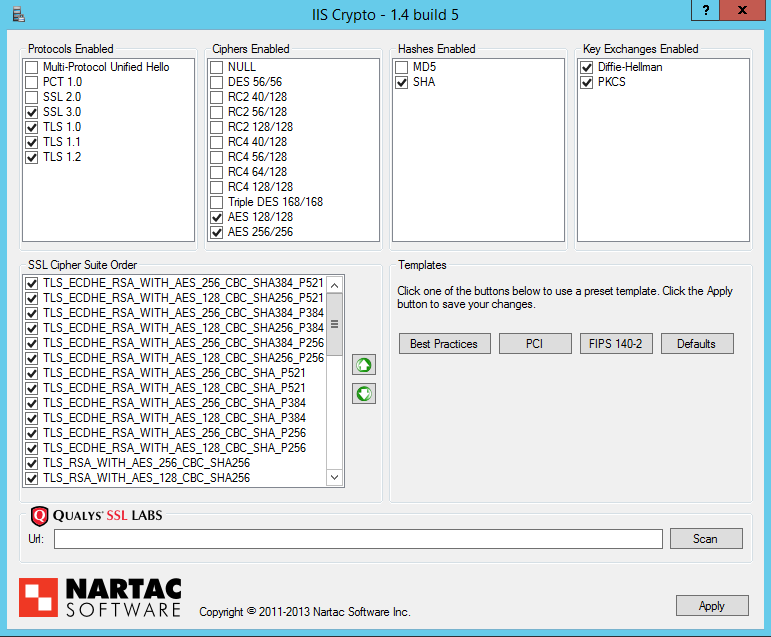
\includegraphics[width=0.411\textwidth]{img/IISCryptoConfig.png}
  \caption{IIS Crypto Tool}
  \label{fig:IISCryptoConfig}
\end{figure}

Instead of using the IIS Crypto Tool the configuration can be set
using the Windows Registry. The following Registry keys apply to the
newer Versions of Windows (Windows 7, Windows Server 2008, Windows
Server 2008 R2, Windows Server 2012 and Windows Server 2012 R2). For detailed
information about the older versions see the Microsoft knowledgebase
article. \footnote{\url{http://support.microsoft.com/kb/245030/en-us}}
\begin{lstlisting}[breaklines]
  [HKEY_LOCAL_MACHINE\SYSTEM\CurrentControlSet\Control\SecurityProviders\Schannel] 
  [HKEY_LOCAL_MACHINE\SYSTEM\CurrentControlSet\Control\SecurityProviders\Schannel\Ciphers] 
  [HKEY_LOCAL_MACHINE\SYSTEM\CurrentControlSet\Control\SecurityProviders\Schannel\CipherSuites] 
  [HKEY_LOCAL_MACHINE\SYSTEM\CurrentControlSet\Control\SecurityProviders\Schannel\Hashes] 
  [HKEY_LOCAL_MACHINE\SYSTEM\CurrentControlSet\Control\SecurityProviders\Schannel\KeyExchangeAlgorithms] 
  [HKEY_LOCAL_MACHINE\SYSTEM\CurrentControlSet\Control\SecurityProviders\Schannel\Protocols] 
\end{lstlisting}

\subsubsection{Tested with Version} 
\begin{itemize*}
  \item Windows Server 2008
  \item Windows Server 2008 R2
  \item Windows Server 2012
  \item Windows Server 2012 R2
\end{itemize*}

\begin{itemize*}
  \item Windows Vista and Internet Explorer 7 and upwards
  \item Windows 7 and Internet Explorer 8 and upwards
  \item Windows 8 and Internet Explorer 10 and upwards
  \item Windows 8.1 and Internet Explorer 11
\end{itemize*}






\subsubsection{Settings}
When trying to avoid RC4 (RC4 biases) as well as CBC (BEAST-Attack) by using GCM and to support perfect
forward secrecy, Microsoft SChannel (SSL/TLS, Auth,.. Stack) supports
ECDSA but lacks support for RSA signatures (see ECC suite
B doubts\footnote{\url{http://safecurves.cr.yp.to/rigid.html}}).

Since one is stuck with ECDSA, an elliptic curve certificate needs to be used.

The configuration of cipher suites MS IIS will use, can be configured in one
of the following ways:
\begin{enumerate}
  \item Group Policy \footnote{\url{http://msdn.microsoft.com/en-us/library/windows/desktop/bb870930(v=vs.85).aspx}}
  \item Registry  \footnote{\url{http://support.microsoft.com/kb/245030 }}
  \item IIS Crypto~\footnote{\url{https://www.nartac.com/Products/IISCrypto/}}
  \item Powershell 
\end{enumerate}


Table~\ref{tab:MS_IIS_Client_Support} shows the process of turning on
one algorithm after another and the effect on the supported clients
tested using https://www.ssllabs.com.

\verb|SSL 3.0|, \verb|SSL 2.0| and \verb|MD5| are turned off.
\verb|TLS 1.0| and \verb|TLS 2.0| are turned on.

\ctable[%
caption={Client support},
label=tab:MS_IIS_Client_Support,
]{ll}{}{%
\FL    Cipher Suite & Client
\ML    \lstinline+TLS_ECDHE_ECDSA_WITH_AES_128_GCM_SHA256+ & only IE 10,11, OpenSSL 1.0.1e
\NN    \lstinline+TLS_ECDHE_ECDSA_WITH_AES_128_CBC_SHA256+ & Chrome 30, Opera 17, Safari 6+
\NN    \lstinline+TLS_ECDHE_ECDSA_WITH_AES_128_CBC_SHA+ & FF 10-24, IE 8+, Safari 5, Java 7
\LL}

Table~\ref{tab:MS_IIS_Client_Support} shows the algorithms from
strongest to weakest and why they need to be added in this order. For
example insisting on SHA-2 algorithms (only first two lines) would
eliminate all versions of Firefox, so the last line is needed to
support this browser, but should be placed at the bottom, so capable
browsers will choose the stronger SHA-2 algorithms.

\verb|TLS_RSA_WITH_RC4_128_SHA| or equivalent should also be added if
MS Terminal Server Connection is used (make sure to use this only in a
trusted environment). This suite will not be used for SSL, since we do
not use a RSA Key.

% \verb|TLS_ECDHE_ECDSA_WITH_AES_128_GCM_SHA256| ... only supported by: IE 10,11, OpenSSL 1.0.1e
% \verb|TLS_ECDHE_ECDSA_WITH_AES_128_CBC_SHA256| ... Chrome 30, Opera 17, Safari 6+
% \verb|TLS_ECDHE_ECDSA_WITH_AES_128_CBC_SHA| ... Firefox 10-24, IE 8+, Safari 5, Java 7

Clients not supported:
\begin{enumerate}
  \item Java 6
  \item WinXP
  \item Bing
\end{enumerate}


\subsubsection{Additional settings}
%Here you can add additional settings
It's recommended to use Strict-Transport-Security: max-age=15768000 
for detailed information visit the
\footnote{\url{http://www.iis.net/configreference/system.webserver/httpprotocol/customheaders}}
Microsoft knowledgebase.

You might want to redirect everything to http\textbf{s}:// if possible. In IIS you can do this with the following setting by Powershell:

\begin{lstlisting}[breaklines]
Set-WebConfiguration -Location "$WebSiteName/$WebApplicationName" `
    -Filter 'system.webserver/security/access' `
    -Value "SslRequireCert"
\end{lstlisting}

\subsubsection{Justification for special settings (if needed)}
% in case you have the need for further justifications why you chose this and that setting or if the settings do not fit into the standard Variant A or Variant B schema, please document this here


\subsubsection{References}
\begin{itemize*}
\item \url{http://support.microsoft.com/kb/245030/en-us}
\item \url{http://support.microsoft.com/kb/187498/en-us}
\end{itemize*}

% add any further references or best practice documents here


\subsubsection{How to test}
See appendix \ref{cha:tools}

%%---------------------------------------------------------------------- 
\subsection{Supporting older clients}
% hack.
\gdef\currentsectionname{Webservers-legacy}

Older clients like Internet Explorer on Windows XP (actually the Windows XP
crypto stack), Java 6 and Java 7 aren't supported by the recommended Variant B
cipher string.
To catch most of those old clients you might use their inability to understand
SNI to create a catchall page with a default SSL server. On the default page
you should provide information about upgrading their browser to the user.
This will not work with Java 7 because Java 7 understands SNI.

\subsubsection{Apache}
% hack.
\gdef\currentsubsectionname{Apache}

Create a default SSL server:

\configfile{ports.conf}{12-13}{SNI for SSL on Apache}
\configfile{000-default-ssl}{2-14}{SNI catchall on Apache}

The catchall virtual server needs to be the first server in the config.
You also should not use snakeoil certificates (as in the snipplet above)
but the very same certificate as you use for the real service. In case you
provide several virtual servers via SNI, the certificate for the catchall page
needs to include all their names.

%\subsubsection{lighttpd}
%% hack.
%\gdef\currentsubsectionname{lighttpd}
%
%\todo{someone needs to write that section or we just omit it}

\subsubsection{nginx}
% hack.
\gdef\currentsubsectionname{nginx}

Create a default SSL server:
\configfile{default}{125-139}{SNI catchall on nginx}

The real service then needs to be in its own server definition omitting the
\texttt{default} keyword in the \texttt{listen} directive.
You should not use snakeoil certificates (as in the snipplet above) but the
very same certificate as you use for the real service. In case you provide
several virtual servers via SNI, the certificate for the catchall page needs
to include all their names.

%%% Local Variables: 
%%% mode: latex
%%% TeX-master: "../applied-crypto-hardening"
%%% End: 
